\part{Class}

\chapter{Introduction}

\section{Overview}

类(class)是一种面向对象计算机编程语言的构造,描述了所创建的对象共同的属性和方法。

类是创建对象的蓝图,其更严格的定义是由某种特定的元数据所组成的内聚的包。

类描述了一些对象的行为规则,而这些对象就被称为该类的实例(instance)。

类有接口和结构,其中:



\begin{compactitem}
\item \textsl{接口描述了如何通过方法与类及其实例互操作;}
\item \textsl{结构描述了一个实例中数据如何划分为多个属性。}
\end{compactitem}



类是与某个层的对象的最具体的类型,而且类还可以有运行时表示形式(元对象),这样就可以为操作与类相关的元数据提供运行时支持。


大多数支持类的编程语言都支持不同形式的类继承,而且许多语言还支持提供封装性的特性(比如访问修饰符)。

类为面向对象编程的三个最重要的特性(封装性、继承性和多态性)提供了实现的手段。

\begin{compactitem}
\item 对象提供了模型化和信息隐藏的好处。
\item 类提供了可重用性的好处。
\end{compactitem}

自行车制造商一遍一遍地重用相同的蓝图来制造大量的自行车,开发人员可以使用相同的类(即相同的代码)来一遍一遍地建立对象。



\section{Abstraction}


在现实世界中,经常有属于同一个类的对象,例如某辆自行车只是世界上很多自行车中的一辆。在面向对象软件中,也有很多共享相同特征的不同的对象—矩形、雇用记录和视频剪辑等,可以利用这些对象的相同特征为它们建立一个蓝图。

对象的软件蓝图就是类,通过类可以定义所有一类对象的变量和方法的蓝图或原型。例如,可以建立一个定义包含当前档位等实例变量的自行车类,这个类也定义和提供了实例方法(变档、刹车)的实现。

\begin{compactitem}
\item 类不是它描述的对象,例如自行车的蓝图不是自行车,对象则是现实世界的电子模型或抽象概念。
\item 抽象类被定义为永远不会也不能被实例化为具体的对象。
\end{compactitem}

实际上,抽象类往往用于定义一种抽象上的概念,在类的继承关系中它往往被定义在较上层的位置。

抽象类与接口存在类似的地方,二者都偏重于对共通的方法和属性进行规约,但是抽象类往往可以规约一个共同的方法和属性时提供一个对他们的实现。

以现实世界为例,"水果"可以算作一个抽象类,"苹果"和"香蕉"则可以作为它的派生类,它们的区别在于"水果"是个概念,它不会有实例,但是"苹果"和"香蕉"则肯定会有实例。

实例变量的值由类的每个实例提供。例如,当创建自行车类以后,必须在使用之前对它进行实例化。



当创建类的实例时,就建立了这种类型的一个对象,然后系统为类定义的实例变量分配内存,这样就可以调用对象的实例方法来实现一些功能。

相同类的实例共享相同的实例方法。除了实例变量和方法,类也可以定义类变量和类方法。

操作系统在第一次在程序中遇到一个类时为这个类建立它的所有类变量的拷贝 - 这个类的所有实例共享它的类变量。


从类的实例中或者从类中都可以访问类变量和方法。类方法只能操作类变量,不必访问实例变量或实例方法。



\section{Encapsulation}

所有的面向对象编程语言都共有这些相同的概念:类、实例、消息传递、方法和继承等。


用户可以从多个角度考虑面向对象编程(尤其是对象),因此在不同的面向对象编程语言中,使用不同的术语来表示相似概念是很普遍的事情。

在面向对象设计中引入了不同的抽象层次,通过这些层次来检查程序,这样从高级抽象的角度可以将对象看作是抽象数据类型的实例。

数据抽象是一种有效的解决问题的方式,它将某些信息有意识地隐藏在程序的某个部分。例如,用户开发的一系列抽象数据类型都可以从两个方面来看待。

与Parnas原则相似,从外部来看,抽象数据类型的客户(用户)只能看到抽象行为的操作集合,作为抽象数据类型的另一接口,定义抽象的实现者通过数据变量可以来维护对象的内部状态。

例如,对于堆栈(Stack)的抽象,用户只能看到合法操作的描述—如push、pop和top。另一方面,实现者需要了解用来实现抽象的具体数据结构,这样具体的细节就被封装在更加抽象的框架中。

\begin{figure}[htbp]
\centering
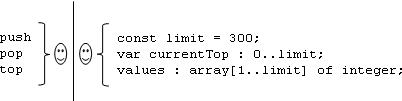
\includegraphics[scale=0.6]{stack.png}
\caption{堆栈的接口和实现}
\label{fig:stack}
\end{figure}

一般使用实例(instance)来表示类的一个具体代表或范例。相应地,使用实例变量(instance variable)来表示实例所维护的内部变量,有时也会使用数据字段(data field)或数据成员(data members)来表示这一概念。

每个实例都有它自己的实例变量集合,客户不能直接改变这些值,只有和类相关的方法才能改变它们。

对象可以简单地看作状态(state)和行为(behavior)的结合,其中状态由实例变量来描述,而行为由方法来表示。

\begin{compactitem}
\item \textsl{从对象外部来看,客户只能看到对象的行为;}
\item \textsl{从对象内部来看,方法通过修改对象的状态以及和其他对象的相互作用来提供适当的行为。}
\end{compactitem}


\chapter{Definition}



\section{Overview}

如果通过在玩纸牌游戏来对纸牌进行抽象,可以通过一系列的细化来扩展纸牌的抽象,其中的每一次细化都会加入少量的新特征。

首先,设想将一张纸牌抽象成一个容器,那么该容器包含纸牌花色和纸牌点数这两个数据值,然后用1~13这些数字来表示纸牌的点数(1代表A纸牌,11、12、13分别代表J、Q和K纸牌)。

\begin{compactitem}
\item 如果使用的编程语言支持枚举(enum),那么可以使用枚举数据类型来表示花色。
\item 如果使用的语言不支持枚举数据类型,则可以使用符号常量和从1~4的整数值来表示花色。
\end{compactitem}


枚举数据类型的优点是可以避免类型错误,因此可以保证一张纸牌的花色一定是四种指定数值之一。如果使用整数来表示花色,就无法防止程序员把无效的整数值赋给纸牌花色变量(例如100)。



下面分别是使用不同语言(C++、Java、C\#)对类的定义的示例。

\begin{lstlisting}[language=C++]
// C++
class PlayingCard {
public:
	enum Suits { Spade, Diamond, Club, Heart };
	
	Suits suit() { return suitValue; }
	int rank() { return rankValue; }
	
private:
	Suits suitValue;
	int rankValue;
};
\end{lstlisting}



\begin{lstlisting}[language=Java]
// Java 
class PlayingCard {
	public int suit() { return suitValue; }
	public int rank() { return rankValue; }
	
	private int suitValue;
	private int rankValue;
	
	public static final int Spade = 1;
	public static final int Diamond = 2;
	public static final int Club = 3;
	public static final int Heart = 4;
}
\end{lstlisting}



\begin{lstlisting}[language={[Sharp]C}]
// C#
class PlayingCard {
enum Suits { Spade, Diamond, Club, Heart };
	public Suits suit() { return suitValue; }
	public int rank() { return rankValue; }
	
	private Suits suitValue;
	private int rankValue;
}
\end{lstlisting}


类的可视性(visibility,又叫可访问性)修饰符(比如public、private等)在C++语言中是用访问修饰符来标明整块说明语句,在Java和C\#中则分别放在每一条语句之前。

在面向对象编程语言中都提供了一种方式用来区别以下这两种情况:一种是可以被类定义的外部(outside)了解和使用的特征,另一种是只能用于类定义内部(within)的特征。其中,后者由关键词private来表示,也就是说使用访问修饰符(public、private等)可以控制类的可视性和可操作性特征。


在C++和C\#语言中,可以定义枚举数据类型来表示纸牌花色。其中,C++语言通过将定义语句放置在类中,可以清晰地表达这两种数据类型之间的联系。

对于C++语言,在类定义之外表示花色的常量必须以类名为前缀:

\begin{lstlisting}[language=C++]
if(aCard.suit() == PlayingCard::Diamond) ...
\end{lstlisting}

对于C\#语言,以枚举类型名为前缀:


\begin{lstlisting}[language=C++]
if(aCard.suit() == Suits.Diamond) ...
\end{lstlisting}

这里,aCard是PlayingCard(纸牌)的一个实例的名称,通过调用suit方法可以检查纸牌的花色。数据字段suitValue和rankValue表示这一抽象的实例数据。每一个PlayingCard类的实例都有自己独立的数据字段,用来维护自己的花色和点数值。

注意,花色值是通过调用suit()这一方法得到的,suit()方法只是简单地返回数据字段suitValue的数值。

大多数语言遵循的惯例是将类名的首字母大写,但并不是所有的语言都这样,尤其是C++程序中更多的是全部使用小写字母来表示类名。


一般情况下,实例变量的命名不需要首字母大写,目的是为了更容易区分类型名和实例变量名。


在Java语言还没有提供枚举数据类型\footnote{从Java 5.0开始引入了枚举类型。}时,通常的做法是定义一系列的符号常量。这里,符号常量需要使用两个修饰符final和static来修饰。

\begin{compactitem}
\item 修饰符final表示这个名称所表示的值不再改变。
\item 修饰符static的意义是不管对这个类创建多少实例,static所修饰的变量实例都只有一个。
\end{compactitem}

final和static修饰符一起作用时,就定义了一个不能改变的唯一变量—也就是常量(constant)。


在使用Java来定义类时,需要注意数据字段suitValue、rankValue和常量Spade、Diamond、Club、Heart之间的区别。其中,后者是由static来修饰的,因此它们存在于任何一个类实例的外部,并且被所有的实例共享,这类似于过程式语言中的全局变量。另外,数据字段suitValue和rankValue不是静态的,因此每个类实例都会有关于这两个数据字段的副本。

Apple公司的Object Pascal语言和Borland公司的Delphi Pascal语言(在Linux平台上称为Kylix)都是基于早期简单的Pascal语言的,因此来自原始语言的很多特征都是一样的,它们都对Pascal语言以各自的方式进行了相应的扩展。

\begin{lstlisting}[language=Pascal]
/* Object Pascal */
type 
	Suits = (Heart, Club, Diamond, Spade);
	
	PlayingCard = object
		suit : Suits;
		rank : integer;
	end;

/* Delphi Pascal */
type 
	Suits = (Heart, Club, Diamond, Spade);
	
	TPlayingCard = class(TObject)
		public 
			constructor Create(r : integer; s : Suits);
			
			function suit : Suits;
			function rank : int;

		private
			suitValue : Suits;
			rankValue : integer;
	end;
\end{lstlisting}



Object Pascal和Delphi Pascal语言都支持枚举数据类型,其中:

\begin{compactitem}
\item 前者使用关键字object来声明一个新类,因此类有时被称为对象类型(object types)。
\item 后者使用关键字class来声明新类,而且要求每一个类都必须从已有的类继承而来,这里通过继承TObject来创建新类。
\end{compactitem}

在Delphi中,类的命名惯例是以大写字母T来开头,而且Delphi语言支持访问修饰符,而Apple语言却不使用访问修饰符。另外,Delphi语言需要构造函数。


Smalltalk语言实际上不使用文本来表示类,而是使用一种称为browser的交互式界面来描述。例如,下图显示了browser的屏幕快照。

\begin{figure}[htbp]
\centering
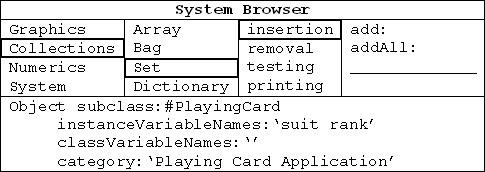
\includegraphics[scale=0.6]{smalltalk_class.jpg}
\caption{Smalltalk浏览器示意图}
\label{fig:smalltalk_class}
\end{figure}

在Browser中,用户通过将消息传递给父类Object来定义一个新类。

与Delphi Pascal语言一样,Smalltalk语言中的所有的类也必须继承于一个特定的父类。例如,上面的示意图说明了包含两个数据字段实例的PlayingCard类的创建。

下面分别是使用其他的不同语言(CLOS、Eiffel、Objective-C)对类的定义的示例。



\begin{lstlisting}[language=Lisp]
// CLOS
(defclass PlayingCard() (rank suit))
\end{lstlisting}






\begin{lstlisting}[language=Eiffel]
// Eiffel
class PlayingCard
feature 
	Spade, Diamond, Heart, Club : Integer is Unique;
	
	suit : integer;
	rank : integer;
end
\end{lstlisting}





\begin{lstlisting}[language={[Objective]C}]
enum suits { Heart, Club, Diamond, Spade };
@ interface PlayingCard : Object
{
	suits suit;
	int rank;
}
@end
\end{lstlisting}



\subsection{C++}




\subsection{Java}





\subsection{Python}


Python语言的格式是逐级缩进的,它不包含用来指示类、函数和语句嵌套的开始和结束符。


\begin{lstlisting}[language=C++]
class PlayingCard:
	"A playing card class"
	def __init__(self, s, r)
		self.suit = s
		self.rank = r
\end{lstlisting}


\subsection{PHP}




\begin{lstlisting}[language=PHP]
class PlayingCard {
	enum Suits { Spade, Diamond, Club, Heart };
	private Suits $suitValue;
	private int $rankValue;
	
	public Suits suit(){
		return $suitValue;
	}
	public int rank(){
		return $rankValue;
	}
}
\end{lstlisting}



\subsection{Ruby}



\begin{lstlisting}[language=Ruby]
class PlayingCard {
	Suits {Spade, Diamond, Club, Heart}
	attr_reader :suitValue, :rankValue;
	def initialize(suitValue, rankValue)
		@suitValue, @rankValue = suitValue, rankValue
	end
	def <=>(card)
		suitValue <=> card.suitValue
		rankValue <=> card.rankValue
	end
	def to_s
		"#{suitValue} (#{rankValue})"
	end
end
}
\end{lstlisting}





\chapter{Method}


\section{Overview}


关于纸牌抽象的进一步改进,包括以下几个方面:

\begin{compactitem}
\item 增加一种方法,可以返回纸牌的颜色(红色还是黑色);
\item 增加一个数据字段,来表示纸牌是面朝上还是面朝下,并且增加检测这一数据字段值状态的方法和翻转纸牌的方法。
\end{compactitem}


使用C\#定义的用来表明这些变化的一个典型的类如下所示:

\begin{lstlisting}[language={[Sharp]C}]
class PlayingCard{
	// constructor, initialize new playing card
	public PlayingCard(Suits is, int ir){
		suit = is;
		rank = ir;
		faceup = true;
	}
	
	// operations on a playing card
	public Boolean isFaceUp(){
		return faceup;
	}
	public Suits suit(){
		return suitValue;
	}
	public int rank(){
		return rankValue;
	}
	public void setFaceUp(Boolean up){
		faceUp = up;
	}
	public void flip(){
		setFaceUp(!faceUp);
	}
	public Color color(){
		if((suit() == Suits.Diamond) || (suit() == Suits.Heart))
			return Colors.Red;
		return Color.Black;
	}
	
	// private data values
	private Suits suitValue;
	private int rankValue;
	private Boolean faceUp;
}
\end{lstlisting}



其中,需要注意的特征就是增加了第二个枚举数据类型来表示颜色,并且又增加了以private来修饰的第3个数据字段来表示纸牌面朝上状态。

将数据字段声明为private意味着禁止从类定义的外部来存取该数据字段,从而确保了修改该数据字段的唯一方式就是使用与这个类相联系的方法。

大多数的面向对象编程方式指南都会建议,数据字段永远不应声明成public,而应该是private或者protected。

构造函数是一种特殊的方法,它们有着和类相同的名称,并且用于在对象中初始化数据字段。

\subsection{getter}


类必须对外提供一种存取数据字段的方法,通过定义于类中的方法来存取数据字段是一种好的面向对象编程方式。

仅仅返回数据字段值的方法称为存取器(accessor),有时也称为获取器(getter)。这里,getter方法的一个实例是isFaceUp,它返回数据字段faceUp的值。另外一个例子是方法rank,它返回数据字段rankValue的值。


为什么对这个简单的行为使用一个方法,而不是直接存取数据字段来实现呢?

一个原因就是方法可以使数据字段是只读的(read-only)。函数只能被调用,而数据字段既可以读又可以写,因此通过private数据字段和public存取器的结合,我们可以确保纸牌的点数一旦创建,就不会被改变。


这里所使用的对方法的命名是一种典型的命名约定。以is开头命名一个返回布尔值的方法是很好的做法,它清楚地表示了当方法返回真值时所代表的含义。按照这一约定,可以更容易理解条件语言中使用的方法,如下所示:

\begin{lstlisting}[language={[Sharp]C}]
if(aCard.isFaceUp())...
\end{lstlisting}


这里,aCard是PlayingCard类的一个实例。很多编程方式指南建议存取器方法以get这个词开始,这样可以清晰地表明,该方法最主要的目的仅仅是获取数据字段的值。这一约定也使得使用这种方法的语句更容易理解,如下所示:



\begin{lstlisting}[language={[Sharp]C}]
int cardRank = aCard.getRank();
\end{lstlisting}

然而,这一约定并不适用于任何情况,尤其是当为这些方法使用更简单的名称rank和suit时。

\subsection{setter}


主要目的仅仅是设置字段值的方法称为可变器(mutator)或者设置器(setter),设置器的命名通常以单词set开始。例如,方法setFaceUp就是设置器的一个实例,它用来设置存取器faceUp的值。


\begin{lstlisting}[language={[Sharp]C}]
class PlayingCard{
	...
	void setFaceUp(Boolean up){
		faceUp = up;
	}
	...
}
\end{lstlisting}

flip方法既不是获取器也不是设置器,因为它既没有获取数据字段值,也没有设置数据字段值。它只是一个简单的方法。方法color从技术上来说也不是获取器,因为它没有获得关于这个类的数据字段值。尽管如此,但由于它返回了对象的一个属性,所以一些编程指南建议,getColor是一个更好的命名。


Smalltalk语言不支持访问修饰符。

缺省情况下,Smalltalk语言中的所有数据字段都是private(即只能在类定义内部进行存取)。为了存取数据字段,必须提供相应的存取器方法:


\begin{lstlisting}[language=bash]
rank 
	" return the face value of a card "
	'$\uparrow$' rank
\end{lstlisting}



Smalltalk语言并没有广泛地遵循以单词get开始的命名约定。通常情况下,Smalltalk语言中存取器方法与它们返回的数据字段同名。

获取器和设置器函数(或者称为存取器和可变器),通过它们可以对数据字段进行存取,这样使用方法而不是直接存取数据字段,用户可以更加灵活地控制数据的修改方式以及确定数据所处的位置。


\section{Declaration}


一般说来,并不指定在类定义中方法的声明次序,只是次序对代码的可读性有很大的影响。

\begin{compactitem}
\item 在类定义中,首先列出一些主要的特征,一些次要的特征列在后面。
\item 构造函数是对象定义的一个最重要的方面,因此应该位于类定义的顶部。
\item 对方法的声明应该通过分组来表示,这样可以迅速便捷地找到对应于给定消息选择器的方法。分组的原则可以按照字母顺序排列,或者按照方法的职能进行分组。
\item 私有数据类型只是对于类的开发者才重要,它们应该列在类定义中靠后的位置。
\end{compactitem}



\section{Constant}

一些编程语言提供了一种方式来作为存取器方法的一种替代,可以指定一个数据字段是变的或者是不可变的。


\begin{lstlisting}[language=C++]

\end{lstlisting}





\begin{lstlisting}[language=C++]

\end{lstlisting}






\begin{lstlisting}[language=C++]

\end{lstlisting}






\begin{lstlisting}[language=C++]

\end{lstlisting}






\begin{lstlisting}[language=C++]

\end{lstlisting}






\begin{lstlisting}[language=C++]

\end{lstlisting}






\begin{lstlisting}[language=C++]

\end{lstlisting}






\begin{lstlisting}[language=C++]

\end{lstlisting}







\begin{lstlisting}[language=C++]

\end{lstlisting}






\begin{lstlisting}[language=C++]

\end{lstlisting}






\begin{lstlisting}[language=C++]

\end{lstlisting}







\begin{lstlisting}[language=C++]

\end{lstlisting}






\begin{lstlisting}[language=C++]

\end{lstlisting}






\begin{lstlisting}[language=C++]

\end{lstlisting}






\begin{lstlisting}[language=C++]

\end{lstlisting}






\begin{lstlisting}[language=C++]

\end{lstlisting}





\begin{lstlisting}[language=C++]

\end{lstlisting}





\begin{lstlisting}[language=C++]

\end{lstlisting}





\begin{lstlisting}[language=C++]

\end{lstlisting}






\begin{lstlisting}[language=C++]

\end{lstlisting}






\begin{lstlisting}[language=C++]

\end{lstlisting}






\begin{lstlisting}[language=C++]

\end{lstlisting}





\begin{lstlisting}[language=C++]

\end{lstlisting}





\begin{lstlisting}[language=C++]

\end{lstlisting}















































